\documentclass{article}
\usepackage{tikz}

\begin{document}

\begin{figure}[htbp]
    \centering
    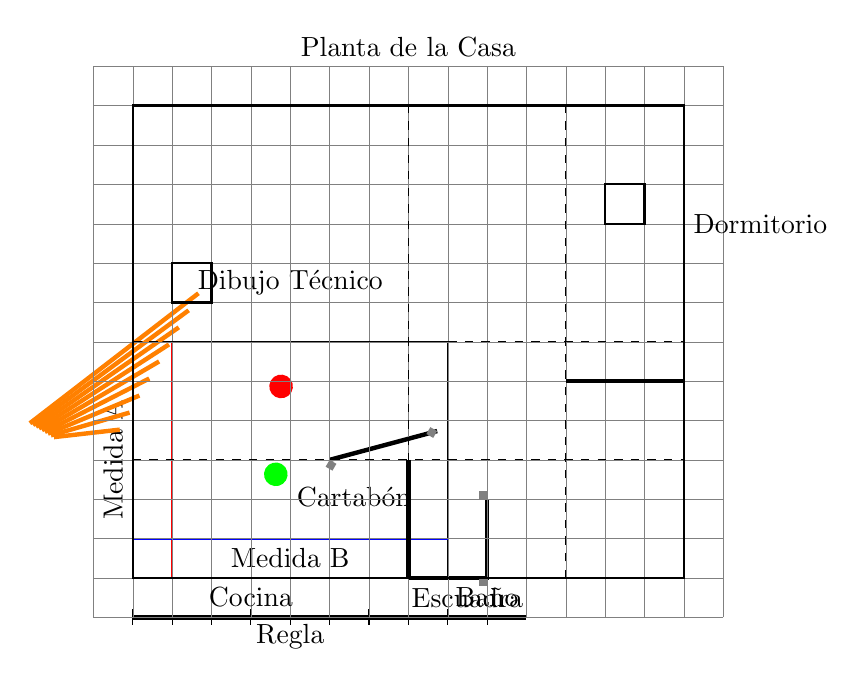
\begin{tikzpicture}[scale=0.5]
        % Líneas guía principales
        \draw[gray,ultra thin] (0,0) grid (10,8);
        % Rectángulo principal
        \draw[thick] (1,1) rectangle (9,7);
        % Líneas adicionales
        \draw[red,thick] (2,1) -- (2,7);
        \draw[blue,thick] (1,2) -- (9,2);
        % Texto
        \node at (5,8.5) {Dibujo Técnico};
        \node[rotate=90] at (0.5,4) {Medida A};
        \node at (5,1.5) {Medida B};
        % Escuadra
        \draw[ultra thick] (8,1) -- (10,1) -- (10,3);
        \fill[gray] (10,1) rectangle (9.8,0.8);
        \fill[gray] (10,3) rectangle (9.8,3.2);
        \node at (9.5,0.5) {Escuadra};
        % Regla
        \draw[ultra thick] (1,0) -- (11,0);
        \foreach \x in {1,2,...,10}
            \draw (\x,0.2) -- (\x,-0.2);
        \node at (5,-0.5) {Regla};
        % Cartabón inclinado y líneas inclinadas
        \begin{scope}[rotate around={-30:(6,4)}]
            % Cartabón
            \draw[ultra thick] (6,4) -- (8,6);
            \fill[gray] (8,6) rectangle (7.8,5.8);
            \fill[gray] (6,4) -- (6.2,4) -- (6.2,3.8) -- (6,3.8) -- cycle;
            \node at (7,3.5) {Cartabón};
            % Líneas inclinadas
            \foreach \y in {2,2.5,...,6} {
                \draw[orange,ultra thick] (1,\y) -- ({\y*tan(170)},1);
            }
            % Círculos
            \fill[green] (5,3) circle (0.3);
            \fill[red] (4,5) circle (0.3);
        \end{scope}

        % Líneas guía principales
        \draw[gray,ultra thin] (0,0) grid (16,14);
        % Rectángulo principal (casa)
        \draw[thick] (1,1) rectangle (15,13);
        % Líneas adicionales para representar las divisiones de las habitaciones
        \draw[dashed] (1,4) -- (15,4);
        \draw[dashed] (1,7) -- (15,7);
        \draw[dashed] (8,1) -- (8,13);
        \draw[dashed] (12,1) -- (12,13);
        % Texto
        \node at (8,14.5) {Planta de la Casa};
        % Etiquetas de habitaciones
        \node[below] at (4,1) {Cocina};
        \node[below] at (10,1) {Baño};
        \node[right] at (15,10) {Dormitorio};
        % Puertas
        \draw[ultra thick] (12,6) -- (15,6);
        \draw[ultra thick] (8,4) -- (8,1);
        % Ventanas
        \draw[thick] (2,8) rectangle (3,9);
        \draw[thick] (13,10) rectangle (14,11);

    \end{tikzpicture}
    \caption{Collage de Dibujo Técnico con Líneas Paralelas Inclinadas y Círculos}
    \label{fig:dibujo_tecnico_circulos}
\end{figure}

\end{document}